% !TEX encoding = UTF-8
% !TEX TS-program = pdflatex
% !TEX root = ../tesi.tex
% !TEX spellcheck = it-IT

%************************************************

%************************************************
\color{red}
Il sistema

-Componenti:

1. Data Cleaning;

2. NLP;

3. Information extraction and entity linking;

4. Clustering:

	- Similarità semantica;
	
    - Similarità sintatica;
   
    - Composizione;
 			

\color{black}

Dato uno stream  di tweet (ordinato temporalmente), l'obiettivo  è quello di individuare dei "topic” o “event”. In letteratura, come già descritto nel capitolo \ref{cap:capitolo2}, esistono due principali metodologie : document-pivot e feature-pivot.
In questo lavoro di tesi, è stata adottata la prima metodologia, l'obiettivo è quindi suddividere lo stream in cluster, tali che ciascuno di essi corrisponda a tutti i tweet relativi ad un \lq\lq evento\rq\rq.  
La definizione di evento utilizzata è quella utilizzata per il Topic Detection and Tracking (TDT) \cite{Allan:2002:TDT:772260} :
In seguito sono descritte in maniera più dettagliata tutte le fasi eseguite.

\begin{figure}[h]
    \centering
    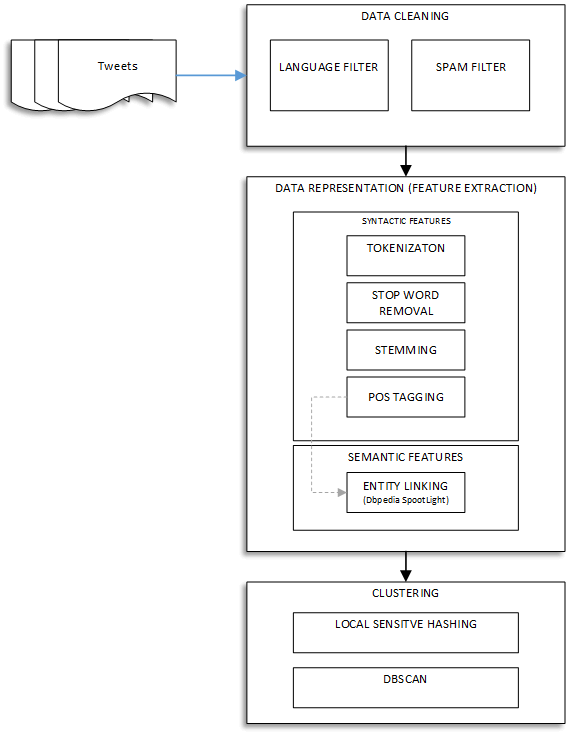
\includegraphics[width=0.6\textwidth]{diagrammaComponenti}
    \caption{Principali componenti del sistema}
    \label{fig:diagrammaComponentiSistema}
\end{figure} 


\section{Data Cleaning: Preprocessing}

Il preprocessing è uno step essenziale per qualunque task di text-mining, quando si ha a che fare con testo derivante dai social media come twitter, tale step diviene di vitale importanza a causa delle caratteristiche dei tweet. In Twitter gli utenti spesso usano slang, abbreviazione e talvolta coniano nuovi termini mai usati 
\`E dunque necessaria una fase accurata di preprocessing per il testo dei tweet prima di poter eseguire qualsiasi modellazione su di essi. 

Il primo passo in questa fase è la rimozione di quelle feature testuali legate ai tweet come:
\begin{itemize}
\item \emph{url:} dal testo sono eliminati tutti i riferimenti a url o media  
\item \emph{@-mentions:} vengono eliminate tutte le mentions ad altri utenti
\item  \emph{\#hashtag:} Per quanto riguarda gli hashtag viene solo eliminato il caratattere   \#   poiché fossero eliminati si potrebbe perdere della semantica dal testo.
Inoltre spesso nei tweet gli hashtag sono composizioni di più parole dove ciascuna parola inizia con una lettera maiuscola (camel Case), come ad esempio \#StopBombingGaza. Gli hashtag che si presentano nella forma su descritta verranno suddivisi nelle parole che di cui sono composti (\#StopBombingGaza $\rightarrow$ Stop Bombing Gaza).
\item \emph{RT:} per i retweet viene considerato il testo del tweet originale.
\end{itemize}
Per il primo passo non è necessaria alcuna fase di parsing del testo poiché tutte queste informazioni sono fornite dalle api di twitter sotto forma di dati strutturati\footnote{nell attributo entities del tweet}.

Molto spesso i tweet sono composti da keywords appartenenti a lingue diverse o contengono caratteri speciali, per tale motivo saranno eliminati tutti i non latin characters \cite{DBLP:conf/msm/BellaachiaA14} . 
 Tramite apposita espressione regolare vengono identificati ed eliminate le emoticons presenti nel testo.
 Una volta terminate queste operazioni di normalizzazione sono stati eseguite due operazioni di filtering:
 \begin{itemize}
 \item language-filtering sono stati considerati solo i tweet in lingua inglese
 utilizzando una libreria open-source scritta in java \footnote{https://code.google.com/p/language-detection/}.
 \item spam-filtering attraverso delle regole euristiche sono stati scartati quei tweet che, potenzialmente, rappresentano spam
 \end{itemize}
 
  
 
Per filtrare  quei tweet che rappresentano potenzialmente dello spam, sono state adottate delle regole empiriche:   \cite{Benevenuto10detectingspammers}
    \begin{itemize}
	\item tweet con più di tre hashtag
	\item tweet con più di due url
	\item tweet con più di tre user-mentions
	\end{itemize}
 


\section{Data Representation} 
Per poter applicare gli algorimi di machine learning è necessario rappresentare gli item attraverso vettori di feature.
I tweet saranno rappresentati come vettori, utilizzando il Vector space Model \cite{Salton:1989:ATP:77013}. 
Il Vector Space Model (VSM), in italiano Modello a Spazio Vettoriale, è una modellazione matematica per documenti testuali che si basa sull'assunzione che il significato dei documenti possa essere rappresentato dai termini che compongono il documento stesso. 
L'intero corpus di documenti, può essere quindi considerato come una matrice $A \in \mathbb{R}^{mxn}$, dove $m$  indica il numero dei termini distinti nel dizionario, $n$  il numero dei documenti 

In questo modello, ciascuna dimensione dei vettori corrisponde ad un termine distinto, e sarà diversa da zero se il termine compare nel documento: i singoli valori $a_{ij}$ della matrice rappresentano il peso
assunto dal i-esimo termine nell’j-esimo documento. Questo peso può essere assegnato in base a  diversi schemi di pesatura, ed è solitamente funzione della frequenza del termine nello specifico documento e di altri fattori, mentre assume valore 0 in assenza del
termine nel documento. Di conseguenza questi vettori sono altamente dimensionali, e molto sparsi dato che i tweet sono composti al più da 140 caratteri. 

\begin{figure}[h]
    \centering
    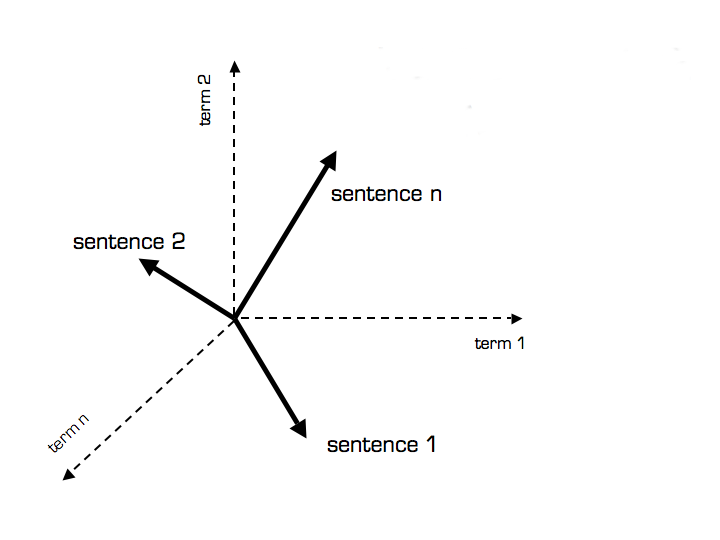
\includegraphics[width=0.6\textwidth]{vector_space}
    \caption{Esempio di documenti in uno spazio vettoriale.}
    \label{fig:dbpedia}
\end{figure}  


Il metodo di pesatura più utilizzato è quello del TF-IDF (Term Frequency-Inverse Document Frequency).
Dato una un termine  $t$, di un documento (tweet) $d$, in una collezione di documenti $D$
che è definita come  
\begin{equation}
tf-idf(t,d, D) =  tf(t,d)\cdot idf(t,D)
\end{equation}
La Term Frequency $tf(w,t)$ è dalla frequenza del termine all'interno del documento. Si presume, che un termine     ripetuto molte volte in un documento, sia molto indicativo del concetto che tale documento vuole esprimere.
Tuttavia vi sono termini che compaiono molto frequentemente in tutti i documenti (come congiunzioni. avverbi che hanno un basso potere informativo).
Per  mitigare questo effetto, viene utilizzato l'Idf che è definito come il logaritmo del rapporto fra numero totale dei documunti nel corpus, e il numero di documenti che contiene il termine $t$.
\begin{equation}
idf(t, D) =  \log \frac{|D|}{|\{d \in D: t \in d\}|}
\end{equation}
L'Inverse Document Frequency   indica la quantità di informazione di un dato termine, ovvero stabilisce se un termine è comune o meno all'interno del corpus. Più il termine è comune minore sarà la sua informazione. 
Poichè si utilizza il logaritmo, se un termine compare in tutti i documenti, il suo valore di Idf sarà pari a 0.

\subsection{Natural Language Processing}
Per poter trasformare il testo in vettori, sono state svolte delle operazioni di Natural Language Processing come:
\begin{enumerate}
\item \textbf{Tokenization}: In questa fase il testo viene suddiviso in unità atomiche dette \emph{token}
\item \textbf{Stop-Word removal}: Rimozione delle parole più comuni nel lessico
\item \textbf{Stemming}: Riduzione di ciascuna parola alla sua radice detta \emph{tema}
\item \textbf{Pos Tagging}: Ad ogni parola viene etichettata con la sua categoria lessicale (Part of Speech).
\end{enumerate}
\subsubsection{Tokenization}

La \emph{Tokenizzazione} è il primo passo di elaborazione di un sistema di Natural Language
Processing. Consiste nella separazione del flusso di caratteri che compone il testo
in input in una serie di elementi atomici detti \emph{token}. I token rappresentano le
unità minime di caratteri consecutivi e possono essere parole, spazio, simboli di
interpunzione e numeri. Sebbene questa operazione di suddivisione in token 
sembrare banale, presenta alcune problematiche. La semplice suddivisione in base allo spazio Suddividere non è sufficiente poiché in molti casi non
ci sono spazi che separano le parole dalla punteggiatura, ci sono sequenze di caratteri senza spazi al loro interno che rappresentano due distinti token (come ad esempio parole precedute da articolo con l'apostrofo, o banalmente parole virgolettate o all'interno di parentesi), esistono sequenze di caratteri. Esistono inoltre molte differenze nelle convenzioni ortografiche, ad esempio nelle date o nei numeri. 
Le tecniche per risolvere questi problemi prevedono l'uso di euristiche ed  espressioni regolari.
 
\subsubsection{Stop-Word Removal}

Le Stop Word sono parole che vengono individuate e filtrate o rimosse all'interno del processo di Natural Language Processing. Solitamente sono contenute in una lista, la stop word list, che può contenere diversi tipi di parole a seconda degli obiettivi dell'applicazione. Solitamente vengono inserite nella lista le parole a più alta frequenza e dunque meno discriminanti, di un certo linguaggio, individuabili dunque all'interno delle categorie chiuse del discorso e tra le parole a maggiore frequenza
delle altre categorie, come ad esempio verbi ausiliari o parole molto generiche. In questo lavoro è stata utilizzata una lista contenente le classiche stopword per la lingua inglese, a cui sono state aggiunte però
delle stopword specifiche per Twitter come: "Retweet","favorite","dm".
\subsubsection{Stemming}
Lo Stemming è il processo di riduzione della forma flessa o derivata di una parola alla sua radice detta \emph{tema}. 
Non è necessario che il tema corrisponda ad una valida radice morfologica, ma è utile che tutte le inflessioni o le derivazioni della parola
vengano ricondotte ad un unico tema, al fine di ridurre complessivamente lo spazio delle parole. 
 Ciò che materialmente gli algoritmi eseguono è la rimozione dei suffissi delle parole, che possono essere enclitici, ovvero essere particelle attaccate alla radice, flessioni che eseguono le declinazioni grammaticali di una parola di una certa categoria e derivazioni che cambiano categoria grammaticale o modificano il significato  

\subsubsection{Pos-Tagging}
 
Il Part of Speech Tagging, che corrisponde in italiano all'analisi grammaticale, consiste nell’associare un'etichetta che si riferisce ad una parte del discorso o categoria lessicale a ciascuna parola in una frase, basandosi sia sulla sua definizione che sul  suo contesto, ovvero la sua associazione rispetto alle parole adiacenti e correlate all’interno di una frase, di un periodo o di un paragrafo.
Le categorie lessicali in italiano sono nove, ovvero verbo, aggettivo, sostantivo,
pronome, articolo, preposizione, avverbio, interiezione e congiunzione, ma possono
variare in altri linguaggi. Cinque di queste parti si dicono variabili perché possono
mutare le loro terminazioni (articolo, nome, aggettivo, pronome, verbo) e quattro
si dicono invariabili perché non possono mutare le loro terminazione: avverbio, pre-
posizione, congiunzione e interiezione. Su di esse si basano i tagset, ovvero insiemi
di etichette che possono essere assegnati alle parole, che possono tenere in consi-
derazione solo la categoria lessicale o anche genere, numero, tempo e così via. I
più utilizzati sono il Penn Treebank   e il Multext.
Processing.
La difficoltà del passo di Part of Speech Tagging consiste nell’ambiguità dell'assegnazione di una specifica etichetta ad una parola, poiché ogni parola può essere
etichettata in diversi modi, potendo essa appartenere a diverse categorie lessicali in base al contesto in cui compare 
Gli algoritmi utilizzati per il Part of Speech Tagging sono principalmente di due
categorie:
\begin{enumerate}
\item \textbf{Basati su regole}  di trasformazione, che impostano le etichette più probabili
per le parole ambigue e successivamente applicano una serie di trasformazioni
apprese da un dataset etichettato per raffinarne i risultati 
\item \textbf{Stocastici} la maggior parte basati su Hidden Markov Model,
che, dopo aver etichettato le parole certe, massimizzano la probabilità che unasequenza di parole abbia una determinata sequenza di etichette utilizzando l'algoritmo di Viterbi \cite{Ryan:1993:VA:901051}.
\end{enumerate}
\end{enumerate}

\subsubsection{Entity Linking} 


 



Il testo del tweet verrà rappresentato con un boosted tf-idf vector utilizzando Apache-lucene\footnote{\href{https://lucene.apache.org/core/}{https://lucene.apache.org/core/}}. 
A partire dal testo dei tweet ripulito, sono state effettuati ulteriori step di nlp come :
\begin{itemize}
\item stop word removal
\item pos tagging (tramite lo stanford pos tagger addestrato su un modello  creato a partire da tweet
\item stemming (o lemmtization)
\end{itemize}
Poich\`e si analizza uno stream di tweet in maniera incrementale è necessario che anche lo schema di pesatura tf-idf sia incrementale ovvero le document-frequencies per una word $w$ variano nel tempo. 

Il peso di una word $w$ di un tweet avente tempo $t$ è dato da:
\begin{equation}
tf-idf_w=tf(w)\ log\frac{N_t}{df_t(w)}boost(w)
\end{equation}
Dove $N_t$ è il numero di tweet al tempo $t$.
Risulta fondamentale assegnare un boost a determinate word poiché, a causa della natura dei tweet (max 140 caratteri), il $tf$ di ciascuna keyword è solitamente pari a 1.  


\begin{equation*}
boost(w):=\begin{cases}
2.0 & \text{se $w$ è un hashtag, on un Proper Nooun}\\
1& \text{altrimenti.}
\end{cases}
\end{equation*}
Solitamente uh hashtag ha un alto potere informativo all’interno di un tweet, nel lavoro di  Phuvipadawat \cite{Phuvipadawat:2010:BND:1913791.1913911}  il boost maggiore per i poper-noun ha prodotto risultati migliori.

\newpage
\section{Semantic Annotation}
Tramite Dbpedia-Spootlight \cite{isem2013daiber} è possibile annotare automaticamente il testo dei tweet con DBpedia URIs.  Ciò permette di arricchire la rappresentazione testuale andando a lenire i classici problemi di ambiguità del linguaggio naturale come polisemia e sinonimia.  
Annotare il testo con DBpedia URis permette di sfruttare la base di conoscenza di DBpedia per poter determinare la correlazione semantica fra due termini. 
Il progetto DBpedia \cite{DBLP:conf/semweb/AuerBKLCI07} oltre a organizzare in maniera strutturata le informazioni di Wikipedia, le collega ad ulteriori open-datasets come: US Census, Geonames, MusicBrainz, the DBLP bibliography, WordNet, Cyc, tramite RDF links come mostrato in figura \ref{fig:dbpedia}  
\begin{figure}[h]
    \centering
    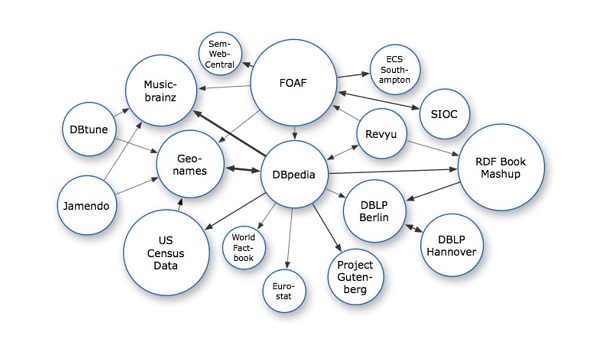
\includegraphics[width=0.6\textwidth]{dbpedia}
    \caption{Datsets interconnessi a DBpedia.}
    \label{fig:dbpedia}
\end{figure}  

Avendo due risorse DBpedia è possibile definire una funzione di distanza, che sfrutti la base di conoscenza di DBpedia. \`E stata definita  una funzione di distanza \emph{Dbpedia Semantic Distance DSD}, che impiega sia DBpedia che il dataset geografico Geonames per risorse di tipo geografico, come segue:
\begin{equation} \label{eq:dbpedia_semantic_distance}
DSD(a,b):=\begin{cases}
GeoDist(a,b) & \text{se $type(a)=location \land type(b)=location$  ,}\\
NDD(a,b) & \text{altrimenti}\\
\end{cases}
\end{equation}
Dove $DSD(a,b) \in [0,1]$,
Milne e Witten \cite{Milne08aneffective} hanno utilizzato gli hyperlink delle pagine Wikipedia per poter definire la correlazione fra due articoli wikipedia (e quindi due risorse dbpedia): date due risorse $a,b$, possiamo definire una \emph{Normalized DBpedia Distance (NDD)} come segue:
\begin{equation} \label{eq:normalized_dbpedia_distance}
NDD(a,b):=\begin{cases}
\frac{\log(max\{|A|,|B|\})-log( |A \cap B|\})}{log(N)-\log(min\{|A|,|B|\})} & \text{se $A \cap B \neq \emptyset $  ,}\\
1 & \text{altrimenti}\\
\end{cases}
\end{equation}
 $A$ e $B$  sono gli insiemi delle risorse DBpedia che hanno un link rispettivamente verso $a$ e $b$, mentre $N$ è il numero totale di risorse in DBpedia. Questa distanza varia nell'intervallo [0,1] dove 1 sta ad indicare che non vi è nessuna correlazione fra i due concetti, mentre 0 indica che i due concetti hanno lo stesso significato. L'idea alla base, è che due risorse saranno simili se esiste una terza che ha un link verso entrambe.
 
 
\section{Clustering}
L'algoritmo di clustering utilizzato è  Dbscan poiché può gestire bene il rumore e non necessita di parametri come il numero di cluster a priori. La distanza utilizzata si basa sia sulla rappresentazione tf-idf del tweet sia sui DBpedia URIs estratti :
\begin{equation}
dist(a,b)=1- timeSim(a,b)\,\frac{textSim(a,b)+semanticSim(a,b)}{2}
\end{equation}
La similarità testuale è data dalla similarità del coseno fra i vettori tf-idf dei due tweet:
\begin{equation*}
textSim(a,b)=\frac{v_a \cdot  v_b}{||v_a||\:||v_b||}
\end{equation*}
 Anche il tempo di creazione dei tweet verrà preso in considerazione per valutarne la distanza, poiché anche se due tweet avessero un testo molto simile es \emph{“tonight  flashmob in central park”}, ma fossero pubblicati ad un mese di distanza, è molto inverosimile che si riferiscano al medesimo evento. Per tale ragione, è stata definita una similarità temporale  \footnote{d$_a$=\#days from the epoch of tweet $a$}
\begin{equation*} 
timeSim(a,b):=\begin{cases}
1-\frac{|d_a-d_b|}{31} & \text{se $|d_a-d_b|<31 $  ,}\\
0 & \text{altrimenti}\\
\end{cases}
\end{equation*}
Ad un tweet, tramite il processo di annotazione semantica, possono essere associate una nessuna o più risorse DBpedia,la distanza semantica sarà data dalla distanza degli insiemi di risorse associati ai due tweet valutata secondo la distanza definita in precedenza per le risorse DBpedia\ref{eq:dbpedia_semantic_distance}. La similarità fra un elemento $x$ e un insieme $Y$ è data da:
\begin{equation*}
	sim(x,Y)=sup\{1-DSD(x,y)\:| y\in Y \}
\end{equation*}

Dati due insiemi di risorse DBpedia $D_a,D_b$ la similarità fra i due insiemi sarà definita come: 
\begin{equation}
sim(D_a,D_b)=\frac{\sum\limits_{x \in D_a} sim(x,D_b)  }{|D_a|} 
\end{equation}

Questa funzione di similarità non è simmetrica,\footnote{se $D_a\subseteq D_b\Rightarrow sim(D_a,D_b)\neq sim(D_b,D_a) $}
Per ottenere una funzione simmetrica è sufficiente definirla come: 
\begin{equation*} 
semanticSim(a,b):= 
\begin{cases}
\frac{sim(D_a,D_b)+sim(D_b,D_a)}{2} & \text{se $D_a,D_b\neq \emptyset$ }\\
1& \text{altrimenti.}

\end{cases}
\end{equation*}
Se ad uno dei due tweet non è associata nessuna risorsa, la similarità semantica sarà pari ad uno, quindi la loro similarità sarà valutata  solo in base alla loro rappresentazione testuale.
Utilizzare una similarità semantica serve ad attenuare il problema della “fragmentation” di cui sono affetti i metodi document-pivot, ovvero utilizzando solo la similarità testuale molti eventi possono essere erroneamente suddivisi in più cluster.  Inoltre Petkos e Papadopoulus \cite{DBLP:conf/www/PetkosPK14}  hanno constato che se due tweet condividono uno stesso URL, o  un tweet e in reply all’altro, allora si riferiscono allo stesso topic/evento.
 
\begin{figure}
    \centering
    \begin{subfigure}[b]{0.45\textwidth}
        \centering
        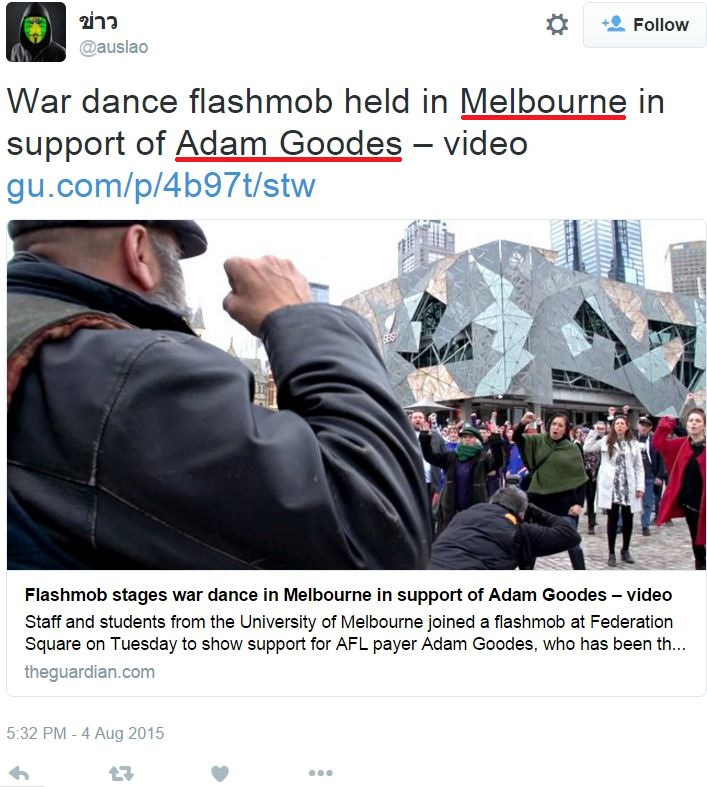
\includegraphics[width=\textwidth]{tweetA}
        \caption{}
        \label{fig:tweeta}
    \end{subfigure}
    \hfill
    \begin{subfigure}[b]{0.45\textwidth}
        \centering
        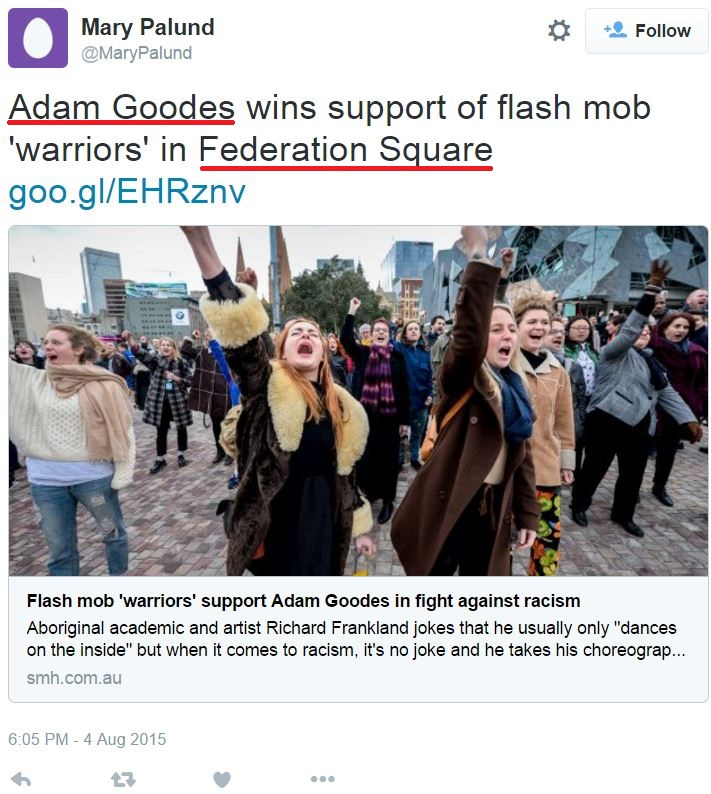
\includegraphics[width=\textwidth]{tweetB}
       \caption{}
        \label{fig:tweetb}
    \end{subfigure}
    \hfill
    
    \caption{Due tweet appartenti allo stesso cluster}
    \label{fig:twotweets}
\end{figure} 
Si considerino i tweet $a,b$ in figura \ref{fig:twotweets}:

\begin{itemize}
\item $textSim(a,b)=0.46$ 
\item $timeSim(a,b)=1.0$ i tweet sono stati pubblicati entrambi il 4/8/2015
\item $semanticSim(a,b):=\frac{sim(D_a,D_b)+sim(D_b,D_a)}{2} $



  $D_a=$\{ \textless\href{http://dbpedia.org/resource/Melbourne}{Melbourne}\textgreater, \textless\href{http://dbpedia.org/resource/Adam_Goodes}{Adam Goodes}\textgreater\}
  
  $D_b=$\{ \textless\href{http://dbpedia.org/resource/Adam_Goodes}{Adam Goodes}\textgreater, \textless\href{http://dbpedia.org/resource/Federation_Square}{Federation Square}\textgreater\}
  
\begin{align*}
 NSD(Melbourne,Adam Goodes)&=NDD(Melbourne,Adam Goodes)\\
 &= \frac{\log(max\{|A|,|B|\})-log(|A \cap B|)}{N-\log(min\{|A|,|B|\})}\\
 &= \frac{\log(643)-log(10)}{N-\log(138)}=0.367  
\end{align*} 
\begin{align*}
 NSD(Melbourne,Federation Square)&=\\
 =GeoDist(Melbourne,Federation Square)&=\\
 =CoordDist(Melbourne,Federation Square) &=0 \: \text{(poichè la distanza in km è 0.8)}
\end{align*}  
\begin{align*}
 NSD(Adam Goodes,Federation Square)=&\\
 NDD(Adam Goodes,Federation Square)&=1 \: \text{poichè} \: A \cap B=\emptyset
\end{align*} 

\begin{align*}
 sim(Melbourne,D_b)&=sup\{1-DSD(Melbourne,y)\:| y\in D_b \}\\
	&=sup\{(1-DSD(Melbourne,Adam Goodes)),\\
	&\:\:\:\:(1-DSD(Melbourne,Federation Square))\}\\
	&=sup\{(1-0.367),(1-0)\}=1	\\	  
 sim(Adam Goodes,D_b)&=sup\{1-DSD(Adam Goodes,y)\:| y\in D_b \}\\
	&=sup\{(1-DSD(Adam Goodes,Adam Goodes)),\\
	&\:\:\:\:(1-DSD(Adam Goodes,Federation Square))\}\\
	&=sup\{(1-0),(1-1)\}=1\\		 
sim(D_a,D_b) &=\frac{1+1}{2}=1 ,\: sim(D_b,D_a) :=\frac{1+1}{2}=1\\
&\implies semanticSim(a,b)=1
\end{align*}
\end{itemize} 
 \begin{align*}
dist(a,b)&=1- timeSim(a,b)\,\frac{textSim(a,b)+semanticSim(a,b)}{2}\\
&=1-\frac{0.46+1}{2}=0.269
\end{align*}

Se invece, $SemanticSim$ fosse definita come la media delle distanze fra tutte le possibili coppie fra i due insiemi avremmo: 

\begin{align*}
	semanticSim(a,b)&=\frac{\sum\limits_{x \in D_a} \sum\limits_{x \in D_b}  (1-NSD(x,y))}{|D_a||D_b|}=\\
	&=\frac{(1-0.36)+(1-0)+(1-0)+(1-1)}{4}=0.73
\end{align*}